\documentclass{article}
\usepackage[utf8]{inputenc}
\usepackage{graphicx}
\graphicspath{ {./imagenes/} }
\usepackage{multicol}
\usepackage[spanish, english]{babel}
\usepackage[left=3cm,right=3cm,top=3cm,bottom=3cm]{geometry}

\providecommand{\keywords}[1]{
  \small	
  \textbf{\textit{\quad \quad Keywords: }} #1}

\providecommand{\pclave}[1]{
  \small	
  \textbf{\textit{\quad \quad Palabras Clave: }} #1}

%Idiomas: \selectlanguage{english} \selectlanguage{spanish}

\begin{document}

\title{Trabajo Encargado N°1: Patrones de Diseño de Software}

\begin{titlepage}
\begin{figure}[htb]
\begin{center}

\includegraphics[width=5cm]{logo.png}
\end{center}
\end{figure}
\vspace*{-0.25in}
\begin{center}
\large{UNIVERSIDAD PRIVADA DE TACNA}\\
\vspace*{-0.025in}
INGENIERIA DE SISTEMAS  \\

\vspace*{0.5in}
\begin{large}
TITULO:\\
\end{large}

\vspace*{0.1in}
\begin{Large}
\textbf{Patrones de Diseño de Software} \\
\end{Large}

\vspace*{0.3in}
\begin{Large}
\textbf{CURSO:} \\
\end{Large}

\vspace*{0.1in}
\begin{large}
CALIDAD Y PRUEBAS DE SOFTWARE\\
\end{large}

\vspace*{0.3in}
\begin{Large}
\textbf{DOCENTE:} \\
\end{Large}

\vspace*{0.1in}
\begin{large}
 Ing. Patrick Cuadros Quiroga\\
\end{large}

\vspace*{0.2in}
\vspace*{0.1in}
\begin{large}

Integrantes: \\
\begin{flushleft}
Garcia Salazar, Briset Celia\hfill(2018062496) \\
Flores Querie, Luis Fernando\hfill(2018062394)\\
Aguilar Soto, Carlos Eduardo\hfill(2017057554)\\
Huallpa Huaychani,Alexander Junior\hfill(2018062497)\\
Paz Huaychani, Kevin Frank \hfill(2019063321)\\
Ticona Chambi, Jhon Thomas \hfill(2018062232)\\

\end{flushleft}
\end{large}

\vspace*{0.1in}
\begin{large}
Tacna - Perú\\
2021
\end{large}
\end{center}
\end{titlepage}

\selectlanguage{spanish}
\begin{abstract}
\quad En el siguiente trabajo se describen los tres principales tipos de patrones de diseño de software (creacional, estructural, comportamiento), cada uno cuenta con diversas formas de aplicación, de estas se colocó un pequeño concepto y en qué situaciones se suele o son adecuadas para aplicar.
Se escogió uno en específico de cada patrón para poder mostrar un ejemplo en aplicación.
\end{abstract}
\pclave{SOLID}

\selectlanguage{english}
\begin{abstract}
\quad The following work describes the three main types of software design patterns (creational, structural, behavior), each one has different forms of application, of these a small concept was placed and in which situations it is usually or is suitable for Apply.
A specific one of each pattern was chosen in order to show an example in application.
\end{abstract}
\keywords{SOLID} 


\begin{multicols}{2}

\section{Introducción}
Los patrones de diseño de software son
soluciones para problemas típicos y
recurrentes que nos podemos encontrar
a la hora de desarrollar una aplicación.
Cada uno de los patrones de diseño han
sido pensados y estructurados tomando
en cuenta las mejores prácticas de
programación y tomando muy en
cuenta los principios SOLID.

\section{Objetivos}
Investigar y conocer más sobre los
principales tipos de patrones de
diseño de software

\section{Desarrollo}
\subsection{Patrones Creacionales}
Los patrones creacionales proporcionan
varios mecanismos de creación de objetos
que incrementan la flexibilidad y la
reutilización del código existente.

\textbf{Abstract Factory}, Es un patrón de
diseño creacional que resuelve el
problema de crear familias enteras de
productos sin especificar sus clases
concretas. Este patron define una
interfaz para crear todos los productos,
pero deja la propia creación de
productos para las clases de fábrica
concretas. Cada tipo de fábrica se
corresponde con cierta variedad de
productos.

Uno de los propósitos de este patrón es:
\begin{itemize}
 \item Proporcionar una interfaz
para crear familias de
objetos relacionados o que
dependen entre sí, sin
especificar sus clases
concretas.

 \item Crear diferentes objetos,
todos pertenecientes a la
misma familia.
\end{itemize}

\textbf{Builder Patterns}, Es un patrón de
diseño creacional que nos permite
construir objetos complejos paso a
paso. El patrón nos permite producir
distintos tipos y representaciones de
un objeto empleando el mismo
código de construcción.

Una de las ventajas de emplear este patrón seria:
\begin{itemize}
 \item Poder construir objetos paso a paso, aplazar pasos de la construcción o ejecutar pasos de forma recursiva.
 \item Poder reutilizar el mismo código de construcción al construir varias representaciones de productos.
 \item Principio de responsabilidad única. Puedes aislar un código de construcción complejo de la lógica de negocio del producto.
\end{itemize}

\textbf{Singleton}, Es un patrón que nos permite asegurarnos de que una clase tenga una única instancia, a la vez que proporciona un punto de acceso global a dicha instancia.
El patrón Singleton resuelve dos problemas al mismo tiempo, estos son:
\begin{itemize}
 \item Garantizar que una clase tenga una única instancia.
 \item Proporcionar un punto de acceso global a dicha instancia.
\end{itemize}
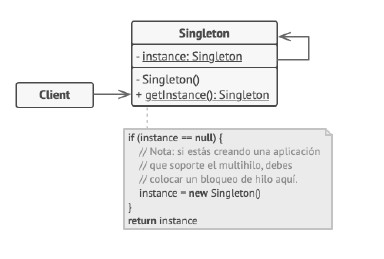
\includegraphics[width=5cm]{imagen1.jpg}

\textbf{Prototype}, Es un patrón de diseño creacional que nos permite copiar objetos existentes sin que el código dependa de sus clases. Delega el proceso de clonación a los propios objetos que están siendo clonados. El patrón declara una interfaz común para todos los objetos que soportan la clonación. Esta interfaz nos permite clonar un objeto sin acoplar el código a la clase de ese objeto. Normalmente, dicha interfaz contiene un único método clonar.

\textbf{Factory Method}, Es un método que nos permite crear instancias de objetos de un tipo determinado,

encapsulando así la creación de dichos objetos. El patrón Factory Method sugiere que, en lugar de llamar al operador new para construir objetos directamente, se invoque a un método fábrica especial.

\subsection{Patrones Estructurales}
Se ocupan de cómo se combinan las clases y los objetos para formar estructuras más grandes. Hacen uso de la herencia para componer interfaces o implementaciones.
Este patrón es particularmente útil para lograr que funcionen juntas bibliotecas de clases desarrolladas de forma independiente.

La siguiente describe la función que cumple este objeto en cada patrón:

\textbf{Bridge}, ETiene como objetivo separar los aspectos conceptuales de una jerarquía de clases de su implementación.


\textbf{Composite}, Proporciona un marco de diseño de una composición de objetos con una profundidad de composición variable, basando el diseño en un árbol.


\textbf{Decorator}, Permite agregar dinámicamente funcionalidades suplementarias a un objeto.


\textbf{Facade}, Tiene como objetivo reagrupar las interfaces de un conjunto de objetos en una interfaz unificada que resulte más fácil de utilizar.


\textbf{Flyweight}, Facilita la compartición de un conjunto importante de objetos con granularidad muy fina.


\textbf{Proxy}, Construye un objeto que se substituye por otro objeto y que controla su acceso.


\textbf{Adapter}
Proposito:
Permite la colaboración entre objetos con interfaces incompatibles.

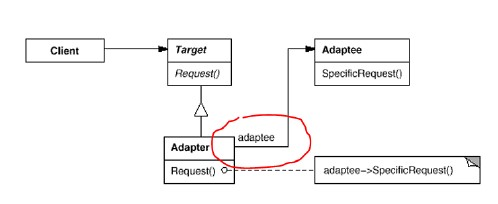
\includegraphics[width=5cm]{imagen2.jpg}

¿Cuándo aplicarlo?
\begin{itemize}
 \item Cuando quieras usar una clase existente, pero cuya interfaz no sea compatible con el resto del código.
 \item Cuando quieras reutilizar varias subclases existentes que carezcan de alguna funcionalidad común que no pueda añadirse a la superclase
\end{itemize}

Ejemplo:
Implementamos una clase que resuelva las fórmulas de una forma geométrica. Funciona perfectamente con un círculo, pero el problema surge cuando intentamos calcular las fórmulas de cuadrado ya que se usan diferentes fórmulas, por eso creamos una clase adapter la cual funcionara como adaptador, este evitara que tengamos la necesidad de crear otra interfaz para la clase cuadrado.

Diagrama de clase:

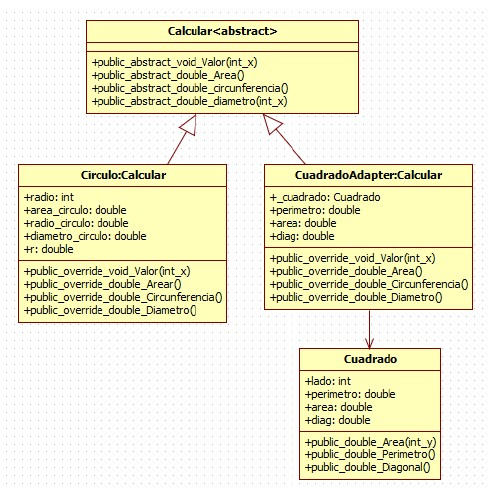
\includegraphics[width=5cm]{imagen3.jpg}

\subsection{Patrones de Comportamiento}
Los patrones de diseño como herramienta de la ingeniería de software, brindan un importante aporte. El estudio de los patrones de comportamiento (según la clasificación Gof) implica conocer la interacción entre los objetos y sus responsabilidades. El presente trabajo propone el uso de perfiles UML y restricciones OCL para la definición de patrones de comportamiento. Dicho enfoque habilita la especificación y validación de patrones tanto en modelos estáticos como dinámicos (Cortez, 2012, p.467).

\begin{itemize}
 \item \textbf{Chain of Responsibility} es un patrón de diseño de comportamiento que te permite pasar solicitudes a lo largo de una cadena de manejadores.
 
 \item \textbf{Command} es un patrón de diseño de comportamiento que convierte una solicitud en un objeto independiente que contiene toda la información sobre la solicitud.
 
  \item \textbf{Interpreter} es un patrón de diseño que, dado un lenguaje, define una representación para su gramática junto con un intérprete del lenguaje. Se usa para definir un lenguaje para construir expresiones regulares que
representen cadenas a buscar dentro de otras cadenas.
  
  \item \textbf{Mediator} es un patrón de diseño de comportamiento que te permite reducir las dependencias caóticas entre objetos.
   
  \item \textbf{Memento} es un patrón de diseño de comportamiento que te permite guardar y restaurar el estado previo de un objeto sin revelar los detalles de su implementación.
    
    \item \textbf{Observer} es un patrón de diseño de comportamiento que te permite definir un mecanismo de suscripción para notificar a varios objetos sobre cualquier evento que le suceda al objeto que están observando.

    \item \textbf{Iterator} es un patrón de diseño de comportamiento que te permite recorrer elementos de una colección sin exponer su representación subyacente (lista, pila, árbol, etc.).
    
    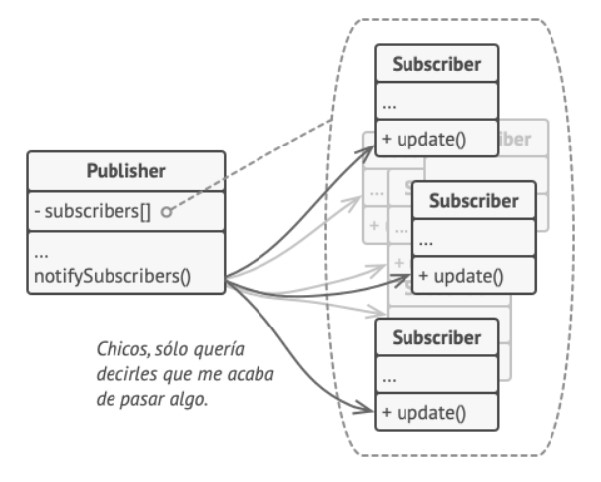
\includegraphics[width=5cm]{imagen4.jpg}

    \item \textbf{State} es un patrón de diseño de comportamiento que permite a un objeto alterar su comportamiento cuando su estado interno cambia. Parece como si el objeto cambiara su clase.
    
    \item \textbf{Strategy} es un patrón de diseño de comportamiento que te permite definir una familia de algoritmos, colocar cada uno de ellos en una clase separada y hacer sus objetos intercambiables.
    
    \item \textbf{Template Method} es un patrón de diseño de comportamiento que define el esqueleto de un algoritmo en la superclase, pero permite que las subclases sobrescriban pasos del algoritmo sin cambiar su estructura.
    
Ayudan a estructurar clases y objetos para poder resolver problemas y, con ello poder adaptarlos al contexto de la aplicación.
Nos permiten crear sistemas con un acoplamiento débil, es decir, orientado a objetos flexibles, que puedan cambiar.
Un sistema bien diseñado será menos propenso a fallos
    
    
\end{itemize}


\section{Conclusiones}
Los patrones de diseño permiten que una parte del sistema varie de forma independiente sin afectar a las demás partes.

Ayudan a estructurar clases y objetos para poder resolver problemas y, con ello poder adaptarlos al contexto de la aplicación.
Nos permiten crear sistemas con un acoplamiento débil, es decir, orientado a objetos flexibles, que puedan cambiar.
Un sistema bien diseñado será menos propenso a fallos

\section{Recomendaciones}
No abuses de los patrones de diseño: no intentes usar un patrón de diseño sólo porque lo conoces, te puede complicar más que ayudar.
Los patrones de diseño son una plantilla de soluciones, los puedes usar adaptándolos a tu problema particular. Pero respetando siempre el concepto sobre el que descansa, si tienes que modificar demasiadas cosas de un patrón para que se adapte a tu problema, quizás sea mejor no utilizarlo.


\end{multicols}

\begin{thebibliography}{XXX0000}
    \bibitem{FRE2014} Shvets, A. (2014). Sumergete en los patrones de diseño [PDF file]. Recuperado de https://refactoring.guru/files/design-patterns-es-demo.pdf.

    \bibitem{DOC2018} Debrauwer, L. (2018). Patrones de diseño en Java. ENI.
    
    \bibitem{FRE2020} 
    Barranco, A. (2020).Software Design Principios y patrones del desarrollo de software [PDF file]. Recuperado de https://www.autentia.com/wp-content/uploads/libros/SoftwareDesignPrincipiosyPatrones-Autentia.pdf
   
    \bibitem{FRE2019} 
    Alejandro, R (2019).Patrones de diseño creacionales. Recuperado de https://ed.team/blog/patrones-de-diseno-creacionales
  
    \bibitem{FRE2009}
    Ralph Johnson; John M. Vlissides (2009) Design Patterns: Abstract Factory. Recuperado de https://www.informit.com/articles/article.aspx?p=1398599
    
    \bibitem{FRE1994}
    Ralph Johnson, John Vlissides (1994). Design Patterns: Elements of Reusable Object-Oriented Software. https://archive.org/details/designpatternsel00gamm/page/97/mode/2up
    
    \bibitem{FRE2012}
    Cortez, A., Riesco, D., & Garis, A. (2012). PERFILES UML PARA LA DEFINICION DE PATRONES DE DISEÑO DE COMPORTAMIENTO. SEDICI. http://sedici.unlp.edu.ar/bitstream/handle/10915/18907/Documentocompleto.pdf?sequence=1&isAllowed=y
    
    \bibitem{FRE2013}
    Belmonte Fernández, Oscar (2013) Concepto de patrones de diseño. Recuperado de http://www3.uji.es/~belfern/Docencia/Presentaciones/ProgramacionAvanzada/Tema2/conceptoPatronDiseno.html#1
    
    \end{thebibliography}

\end{document}